% XeLaTeX can use any Mac OS X font. See the setromanfont command below.
% Input to XeLaTeX is full Unicode, so Unicode characters can be typed directly into the source.

% The next lines tell TeXShop to typeset with xelatex, and to open and save the source with Unicode encoding.

%!TEX TS-program = xelatex
%!TEX encoding = UTF-8 Unicode

\documentclass[12pt]{article}
\usepackage{geometry}   
\geometry{letterpaper}   
%\geometry{landscape} 
\usepackage[parfill]{parskip} 
\usepackage{graphicx}
\usepackage{amssymb}

% Will Robertson's fontspec.sty can be used to simplify font choices.
% To experiment, open /Applications/Font Book to examine the fonts provided on Mac OS X,
% and change "Hoefler Text" to any of these choices.

\usepackage{fontspec,xltxtra,xunicode}
\defaultfontfeatures{Mapping=tex-text}
%\setromanfont[Mapping=tex-text]{Hoefler Text}
%\setsansfont[Scale=MatchLowercase,Mapping=tex-text]{Gill Sans}
%\setmonofont[Scale=MatchLowercase]{Andale Mono}
\setromanfont[Mapping=tex-text]{Times New Roman}
\setsansfont[Scale=MatchLowercase,Mapping=tex-text]{Arial}
\setmonofont[Scale=MatchLowercase]{Courier New}


\title{Emergency Coronavirus Surveillance Opportunities\\[10pt] \large{Community Serosurveillance in USA (and Elsewhere)\\ and Verbal Autopsy Globally}}
\author{Sam Clark\thanks{Thanks to Sara Curran (UW), Richard Li (Yale), Patrick Gerland (UNPD), Shripad Tuljapurkar (Stanford), and Stephan\'e Helleringer (JHU) for commenting on version 1.}\\
The Ohio State University, clark.2962@osu.edu\\
www.samclark.net, work@samclark.net\\
Cell: 206-303-9620}
\date{March 23, 2020}      

\begin{document}
\maketitle


\section{Introduction}

The novel coronavirus pandemic is ravaging the globe, and there are few reliable data to describe basic epidemiology anywhere -- \textit{including the United States}.  Beyond this critically urgent, local need within the communities where we live, as the pandemic gets under way in Africa and other parts of the developing world, there will be very few or no real data on epidemiology, morbidity, or mortality.  The following two ideas contribute to addressing these needs by developing rapid surveillance assessment tools and evidence to address this crisis in the USA and globally, as well as lay the foundation for such surveillance capacities during likely future pandemic crises.


\section{Community Surveillance}

Like most of us who do epidemiology in one form or another, I have saturated myself in news of the pandemic since mid February.  There have been myriad missteps and missed opportunities on the part of our national leadership, but among the most harmful is not having set up an accurate way of assessing the underlying prevalence, and hence the size, scope, and dynamics of the epidemic.  The mainstream media discussion often centers around a lack of testing among those who present with symptoms and their personal contacts.  As any epidemiologist will tell you, limiting testing to those with symptoms and those in their recent social network does not generate accurate prevalence estimates.  Instead, what is needed is a systematic, structured approach to assessing population prevalence that is cheap, fast, and feasible enough to give us effectively real-time tracking of population prevalence.  What we need is the epidemiological equivalent of a political poll, and we need to keep re-polling frequently for the foreseeable future.

While the current situation presents unique challenges and requires a timely response, many of the components we require exist and are widely used in other contexts (e.g. population prevalence of HIV) in the developing world.  Specifically, the key features are (i) lightweight, but representative sampling design and (ii) ability to collect biological specimens. The Demographic and Health Surveys (DHS) conducted by USAID have both of these features, with `biomarker modules' that collect specimens for testing.  Further, the system needs to be transferrable across multiple The actual methodology is complex and requires specific expertise at every stage -- \textit{notwithstanding the complexities, the point is that we already know how to do this, how to design and implement complex sample surveys with biomarkers, and how to analyze the results.}

To address the gaping chasm of evidence that is our current understanding of coronavirus epidemiology in the United States, \textit{I propose leveraging the expertise in collecting surveys with complex designs and biomarker data from the developing world to immediately design and begin implementing a coronavirus sample survey in the most critically affected communities in the United States.}  

\textbf{The immediate aim is to estimate and track over time with scientific confidence the population prevalence of coronavirus disaggregated by age, and as time goes by, as many other useful dimensions as we can afford.}

\subsection{Very brief overview of what is required.}
\begin{itemize}
\item Cooperation and close liaison with local health departments to clearly communicate the usefulness of this approach -- \textit{because real prevalence data to track the epidemic requires a minimum number of tests and person-time to obtain, this need for data collection resources and people must not come at the expense of immediate needs for PPE, testing, and care provision for the vulnerable.} 
\item Cooperation between public health and medicine schools and population health scientists across the nation through existing research infrastructures and research networks -- funded by NIH and NSF.
\item Survey design -- statistical sampling frames and survey design require \textit{power calculations that define the number of tests required for a given level of confidence interval estimates.} Additionally, to increase efficiency, the sampling will likely need to be stratified to increase the likelihood of finding positive cases. 
\item Survey implementation -- survey teams with interviewers and appropriate medical personnel to collect samples (maybe nurse trainees or some other group who are not required as frontline medical workers).
\item Analysis and dissemination of results -- biostatisticians and public health experts to produce results and clearly communicate them to key decision makers.
\end{itemize}

\subsection{Costs.}

It is very hard to judge the costs precisely at the moment, but undoubtedly the total cost will be significant. However, I believe it would be possible to harness the required technical expertise very quickly. It may take slightly more effort to assemble the survey implementation team, but if we were to get started on both immediately, the implementation team could be online at about the time the design team is done with their work. \textit{It can be done.}

The bottom line is that the resulting information would be \textit{invaluable} -- worth the cost whatever it turns out to be.


\section{Verbal Autopsy Globally}

The coronavirus epidemic in the developed world is very grim, and it is just getting underway in much of the developing world.  Given that the developed world is effectively not coping with their epidemics, \textit{the most likely future for the developing world is catastrophic.}  I have one idea that may help provide some valuable tools immediately and over the medium term to provide at least some sense of the burden of disease and how it is affected by the epidemic.

`Verbal autopsy' (VA) is an old method used primarily in research settings to ascertain cause of death using an in-person interview with the caregivers of a recently deceased person.  The interview elicits information on the history of the illness or condition leading up to death including both yes-no questions and often a free-text narrative account of the death.  These data are reviewed either by physicians or computational and statistical algorithms to identify a cause(s) of death that is consistent with the information obtained in the VA interview.  As a means of ascertaining cause of death, VA is, not in fact, very good, but for many people living in populations with no alternative, it is the only feasible approach.  

Recently VA has received a great deal of attention in the context of rapidly improving civil registration and vital statistics systems in the developing world where traditional medical certification and autopsy are not available, or indeed feasible at all.  To address this much larger, routine mortality and cause of death surveillance need, VA is being rapidly improved and adapted to work at scale.  This mainly involves improving the computational and statistical algorithms that process the data in an automated way -- fast, efficient, cheap, and comparable -- and the software that implements the methods and integrates them into existing data systems -- district, province, and national scale. Globally, two groups have contributed important advances in this regard -- a group of collaborators at \textit{IHME and the University of Melbourne}, and the \textit{openVA Team} that I lead.  Likewise, there are two widely used standard toolsets for VA, one developed and maintained by the IHME/Melbourne team, and the other developed and maintained over a longer period of time by the WHO Reference Group on VA, of which I am a key member.  There is a developing consensus among institutional users of VA (i.e. countries) that the WHO toolset is preferable in the long run because it often produces better results and is backed by an institution that has and is very likely to continue supporting it for a very long time.

The most important impediment to rapidly improving VA overall is the need for much more and much better \textit{training data} consisting of a large collection of \textit{reference deaths} that have both VA and a separate cause assigned through an independent mechanism.  These deaths can be used to create \textit{symptom-cause-information} (SCI) that is at the heart of all of the algorithmic approaches to assigning causes using VA data. Collecting labeled data (physical autopsies) is expensive or impossible in the VA context, so practitioners typically make predictions using models trained on other geographic locations.  Figure~\ref{fig:vizpic}(a) uses rare ``gold standard'' data from The Population Health Metrics Research Consortium (PHMRC). These data consist of about 8,000 deaths where each death has both a physical autopsy and a VA survey administered to a caregiver.  
 \begin{figure}
   \begin{center}
      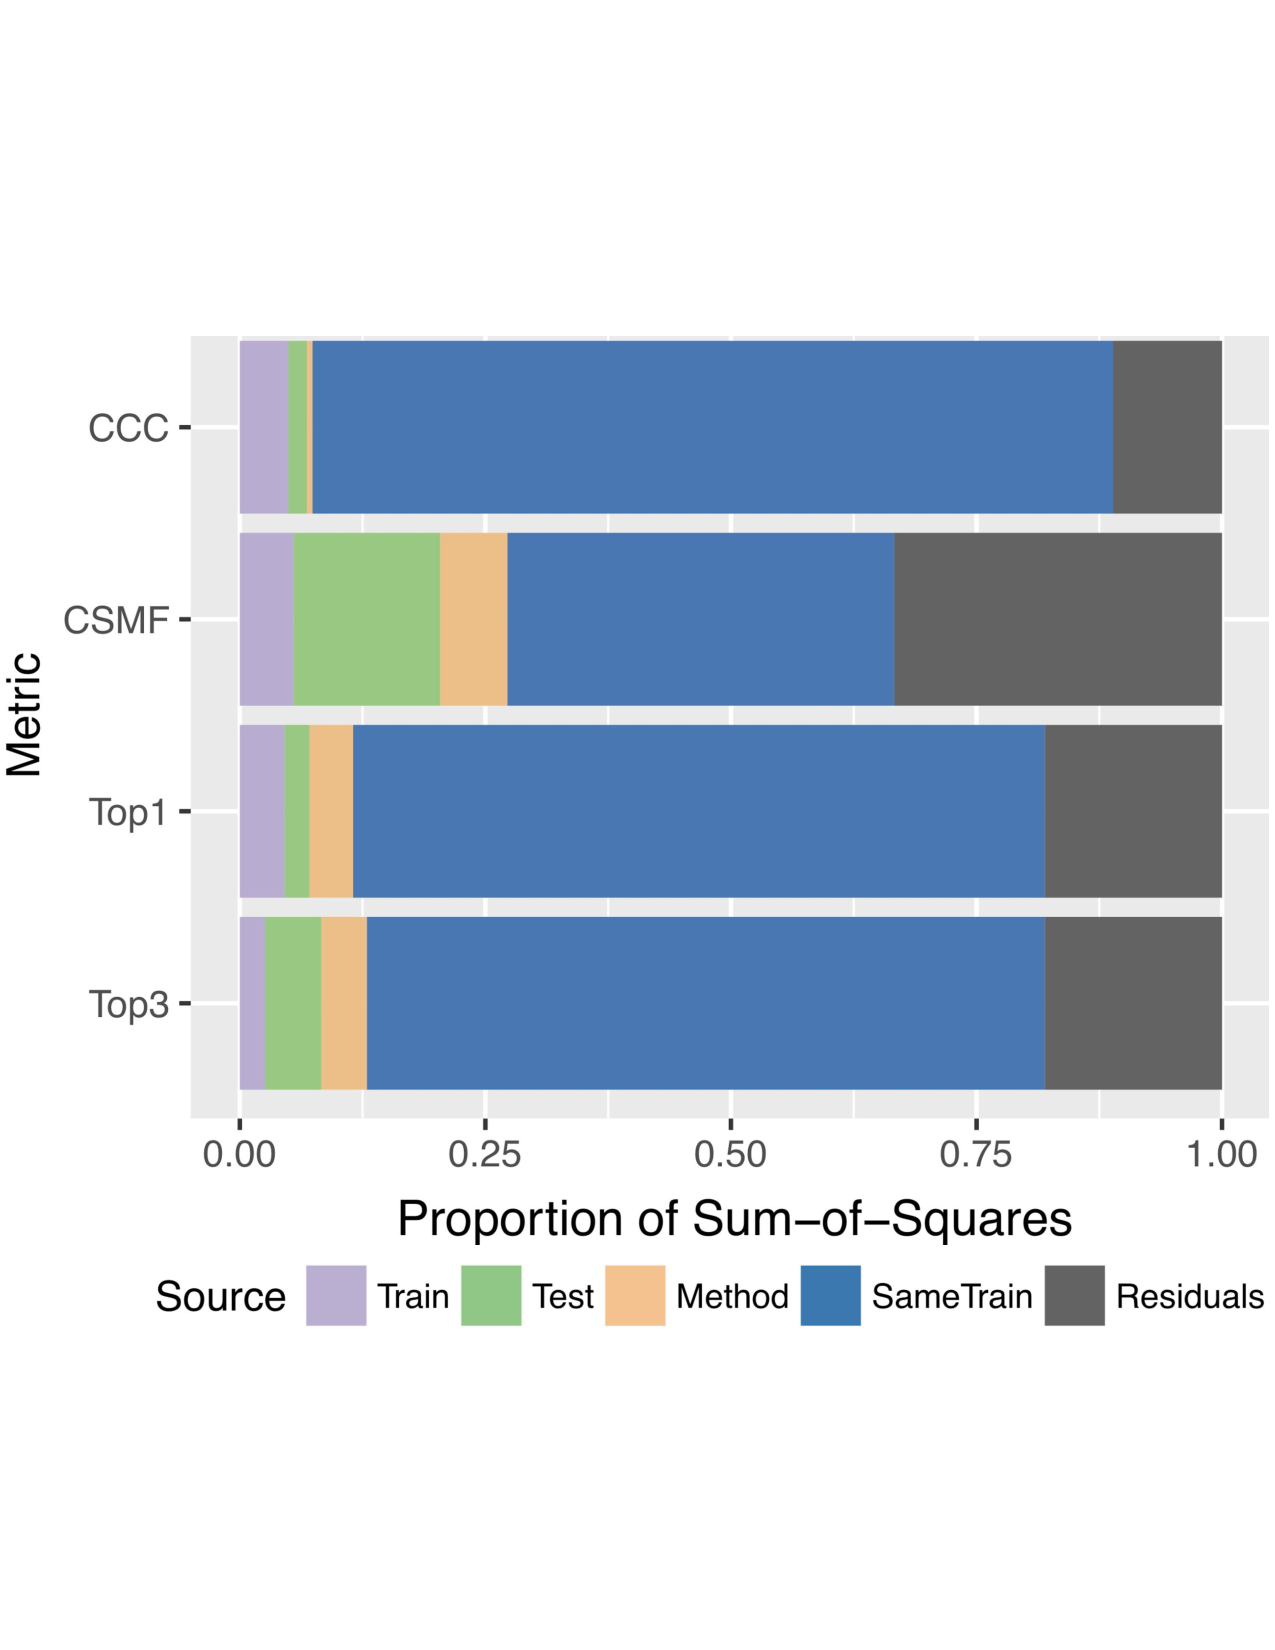
\includegraphics[width=.6\textwidth]{figures/vizpic.pdf}~\\~\\
         \caption{\label{fig:vizpic} The plot represents a decomposition of variability in the outcome of extrapolation for cause of death assignment for VAs.  Each bar represents 100\% of the variation in one particular performance metric.}
   \end{center}
\end{figure}

If extrapolation across geographic areas is reasonable for VA cause of death assessment, then we should be able to make statements like ``Given that someone reporting chest pain and a family history of heart disease in Tanzania was medically shown to have died of a heart attack, we can assume that someone reporting chest pain and a family history of heart disease in India \textit{also} died of a heart attack.'' The PHMRC data come from six different geographic regions across Africa, Latin America, India, and Asia, so we can evaluate this statement by 
using each of the six sites as the ``training phase'' from Figure~\ref{fig:extrapfig} and then applying the prediction function to held out data from all of the sites. Each bar in Figure~\ref{fig:vizpic} contains 100\% of the variation in one of four performance measures commonly used in the literature.  Across all four, the largest driver of variation is whether the method was tested and trained on the same geographic area (blue bar).  These results are not because of differences in the distribution of outcomes, which do exist but have been controlled for here.  Other factors, such as which of five machine learning methods we chose made minimal difference.  In the case of VA, therefore, {\bf developing new machine learning or statistical methods for prediction matters substantially less than collecting relevant data}.  

At this exact moment there is an opportunity in Brazil to both play an important role in developing data on the coronavirus epidemic and get a giant head start on developing a large reference death data set.


\subsection{Specific context in Brazil.}

The Brazilian vital statistics system processes deaths in two streams: 1) external causes are determined by the police, and 2) all other `natural' causes go through a separate system that uses medical certification, autopsy, and in some cases other approaches to determine cause of death.  For a number of years VA has been part of the second system when the other procedures are not possible or when more information is required.

To settle on the cheapest and most accurate best practice for natural causes, the University of Sao Paulo (USP) Department of Pathology has been doing VAs in addition to the other approaches and doing research to greatly improve the utility and cost of so-called needle biopsies or `minimally-invasive autopsies' (MIA).  MIAs consist of tissue sample collected with a large bore needle instead of a full autopsy.

Over the past six months my team has been planning a study with the USP group that would roll out WHO standard VA to 12 sites within Brazil, including Sao Paulo, and combine that with traditional autopsy and MIA to:
\begin{itemize}
\item improve the MIA protocol and develop a companion training course for pathologies,
\item rapidly develop a reference death dataset for the WHO toolset, and
\item greatly improve the overall performance of the system to identify causes of death.
\end{itemize}
Upon completion of the work, we hope to be able to roll out at a national scale a much improved protocol for assigning natural causes of death in Brazil \textit{and have a very greatly improved reference death dataset that can be used to improve VA cause-assignment algorithms for use globally.}  A final benefit will likely be a robust protocol for cheap, feasible MIAs that can be transferred to other countries in Africa and elsewhere.

\subsection{Brazil and the coronavirus.}

There is an extremely time-sensitive opportunity in Brazil that will expire within a few days.  With a comparatively small investment \textit{right now} it will be possible to: 1) greatly improve Brazil's ability to monitor the coronavirus epidemic and the burden of disease generally both now and into the distant future, and 2) \textit{critically}, enable us to rapidly improve the VA method in general so that we can apply it to coming coronavirus epidemics elsewhere and to monitoring the burden of disease globally into the future.  

On Thursday of last week we learned that the State of Sao Paulo in Brazil (the most populous state) is very seriously considering a restructuring of its cause of death system during the coronavirus epidemic.  This will very likely entail converting the existing natural causes system \textbf{to only use VA combined with MIA} because the autopsy and medical certification systems are very likely to not be able to keep up.  \textit{A final decision is scheduled to be made on Tuesday March 24.}  

As of this moment, the Brazilians are using the PHMRC short form VA developed for very rapid, routine mortality surveillance in developing countries. This questionnaire has very few questions and does not perform well in a general sense. To accommodate the uncertain scope of symptoms and overall patterns of death that we are likely to begin seeing very soon in Brazil, we would like to switch to the WHO standard instrument that contains about twice as many questions and is much less likely to omit a critical question. 

This provides a once-in-a-lifetime opportunity to rapidly build up a reference death dataset consisting of WHO standard VAs combined with MIAs, and perhaps later on, with physician coding.  Immediately after the acute coronavirus epidemic subsides, the system will likely continue in some form and again have traditional autopsy. This sequence of events is likely and will include many 100,000s of deaths and perhaps even more over the coming 1--2 years.  The reference death dataset will enable us to rapidly improve the overall performance of VA in Brazil and globally -- where I am very confident VA will play a critical role in measuring and monitoring the burden of disease in Africa (at least).

\subsection{What is required.}

What is required immediately -- within the next 1--2 weeks -- is funds to support programmers to rapidly implement the WHO VA questionnaire with the existing Brazilian VA software system that has been developed and maintained by the USP pathology group.  Because of the very, very short timeframe in which the key decisions will be made, this is extremely urgent.  Specifically, these are the immediately required tasks:
\begin{itemize}
\item translate/adapt WHO standard questionnaire to Portuguese,
\item create an electronic version of the Portuguese WHO questionnaire that is compatible and integrated with the existing system in Brazil, and
\item coordinate with the USP pathology group who will be in charge of implementing the new system to train and roll out the WHO questionnaire.
\end{itemize}
We are working on translating the questionnaire right now, and there is a team of programmers who maintain the existing system standing by to begin the programming task if support for their work becomes available.  

I do not have an accurate assessment of the total cost involved, but from experience, I believe that \$50,000 -- \$100,000 is immediately required to accomplish the first crucial step of getting the system to use the WHO standard tools.  

Fully realizing the benefits of this opportunity will require additional investment, and a careful plan for the near and medium-term future can be made immediately following this initial work. 

\end{document}  





















